\chapter{Constraints}

Bei vielen Problemen gibt es Abh�ngigkeiten in den L�sungskomponenten. Es gibt zum Beispiel F�lle, in denen wenn X den Wert A hat dann hat Y den Wert B. Oder wie im Spiel Sudoku kann dieselbe Zahl nicht zweimal in derselben Reihe oder Diagonale vorkommen. Probleme, bei denen Constraints eine Rolle spielen, und wie sie gel�st werden k�nnen, werden in diesem Kapitel behandelt.

\section{L�sen von Constrain-Problemen}

\paragraph{Allgemeines Constraint Solving Problem}

Bei einer gegebenen Menge von Variablen innerhalb eines bestimmten Wertebereichs und einer Menge von Beschr�nkungen erlaubter Kombinationen der Variablenwerte wird nach einer konkreten Anordnung der Variablen gesucht, die alle Beschr�nkungen erf�llen kann.

\paragraph{Constraint Solving Problem als Suche}

Solche Probleme k�nnen als Suchproblem dargestellt werden, wobei:
\begin{itemize}
    \item \textbf{Suchraum:} Menge von Variablen und derren Dom�nen
    \item \textbf{Anfangszustand:} Alle Variables sind noch unbelegt
    \item \textbf{Zielzustand:} alle Variablen belegt und Constraints erf�llt
    \item \textbf{Zieltest:} �berpr�fe, ob alle Variablen die Constraints erf�llen
\end{itemize}

\subsection{Ans�tze z�r L�sung von Constraint Solving Problemen}

\paragraph{Ansatz 1: Generiere und Teste}

Generiere Kombinationen von Werten f�r die Variablen basierend auf ihren Dom�nen und teste, ob die Bedingungen erf�llt sind. Wiederhole so oft wie n�tig.


\begin{table}[H]
    \centering
    \begin{tabular}{|l|l|l|l|}
    \hline
    \(x_1\) & \(x_2\) & \(x_3\) & \textbf{Test} \\ \hline
    1           & 1           & 1           & nein          \\ \hline
    1           & 1           & 2           & nein          \\ \hline
    1           & 2           & 1           & nein          \\ \hline
    1           & 2           & 2           & nein          \\ \hline
    2           & 1           & 1           & nein          \\ \hline
    2           & 1           & 2           & nein          \\ \hline
    2           & 2           & 1           & ja            \\ \hline
    \end{tabular}
    \caption{\label{tab:generate-and-test} Ergebnis des Generierens und Testens}
\end{table}

\paragraph{Ansatz 2: Tiefensuche mit Backtracking}

Die Werte f�r die Variablen werden systematisch generiert, um nicht alle m�glichen Kombinationen generieren zu m�ssen.

\begin{table}[H]
    \centering
    \begin{tabular}{|l|l|l|l|}
    \hline
    \(x_1\) & \(x_2\) & \(x_3\) & \textbf{Test} \\ \hline
    1           & 1           & 1           & nein          \\ \hline
    1           & 1           & 2           & nein          \\ \hline
    1           & 2           & 2           & nein          \\ \hline
    1           & 2           & 1           & nein          \\ \hline
    2           & 2           & 1           & ja            \\ \hline
    \end{tabular}
    \caption{\label{tab:deepsearch-and-backtracking} Ergebnis von Tiefensuche und Backtracking}
\end{table}

Durch den Einsatz von Heuristiken und anwendungsspezifischen Merkmalen kann die L�sung von Constraint-Problemen effizienter gestaltet werden. Unter Verwendung von Constraints kann der Zustandsraum umstrukturiert werden, um die Constraints zum leichteren L�sen des Problems auszunutzen.

\subsection{Optimierung der L�sung von Constraint Problemen}

Die folgenden Optimierungen lassen sich anhand eines konkreten Beispiels besser erkl�ren. Ein Beispiel f�r ein Problem mit Cosntraints ist die Einf�rbung von Staaten in Australien mit drei Farben, so dass benachbarte Staaten niemals dieselbe Farbe haben.

\begin{figure}[H]
    \centering
    
\includegraphics[width=0.6\textwidth]{figures/kap5/australia-map.png}
    \caption{Karte der Staaten von Australien}
    \label{fig:constraints-australia-states}
\end{figure}

\paragraph{Anwendung von Constraint Netzen}

Ein Netz kann erstellt werden, wenn Probleme bin�re Beschr�nkungen haben. Die Variablen sind die Knoten und die Kanten verbinden die Knoten mit Nebenbedingungen.

\begin{figure}[H]
    \centering
    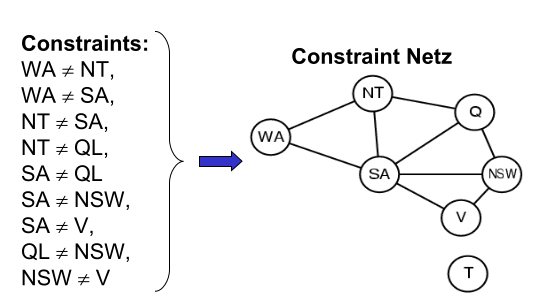
\includegraphics[width=0.6\textwidth]{figures/kap5/australia-constraint-net.png}
    \caption{Constraints-Netz}
    \label{fig:constraint-net-australia}
\end{figure}

Das Constraints Netz kann in Heuristiken verwendet werden, um die Nutzung der Tiefensuche mit Backtracking zu verbessern.

\paragraph{Abalauf von Tiefensuche mit Backtracking zur L�sung von Constraint Problemen}

Mit Hilfe einer \textbf{Degree Heuristik}, bei der mit der Variable begonnen wird, die die meisten Constraints aufweist, kann die Suche optimiert werden. Based on the Constraint Netz in Abb.~\ref{fig:constraint-net-australia}, k�nnen wir sehen, dass SA die meisten Einschr�nkungen hat und die Suche damit beginnen sollte. Danach wird die Suche wie eine typische Tiefensuche (siehe Abschnitt~\ref{section:depth-search-backtracking}) fortgesetzt:-

\begin{enumerate}
    \item In jedem Schritt wird einer Variablen ein Wert zugeordnet.
    \item Wenn die Variable nicht mehr so erweitert werden kann, dass sie den Beschr�nkungen entspricht, wird ein Backtracking durchgef�hrt.
\end{enumerate}

Eine weitere Heuristik, die verwendet werden kann, ist die Minimum-Remaining-Value-Heuristik. 

\section{Vertiefungsprojekt: N-Damen Problem mittels Choco-Solver}

Um besser zu verstehen, wie Constraint-Probleme mit konventionellen Programmiersprachen gel�st werden, wurde das N-Queen-Problem in Java implementiert.

\begin{figure}[H]
    \centering
    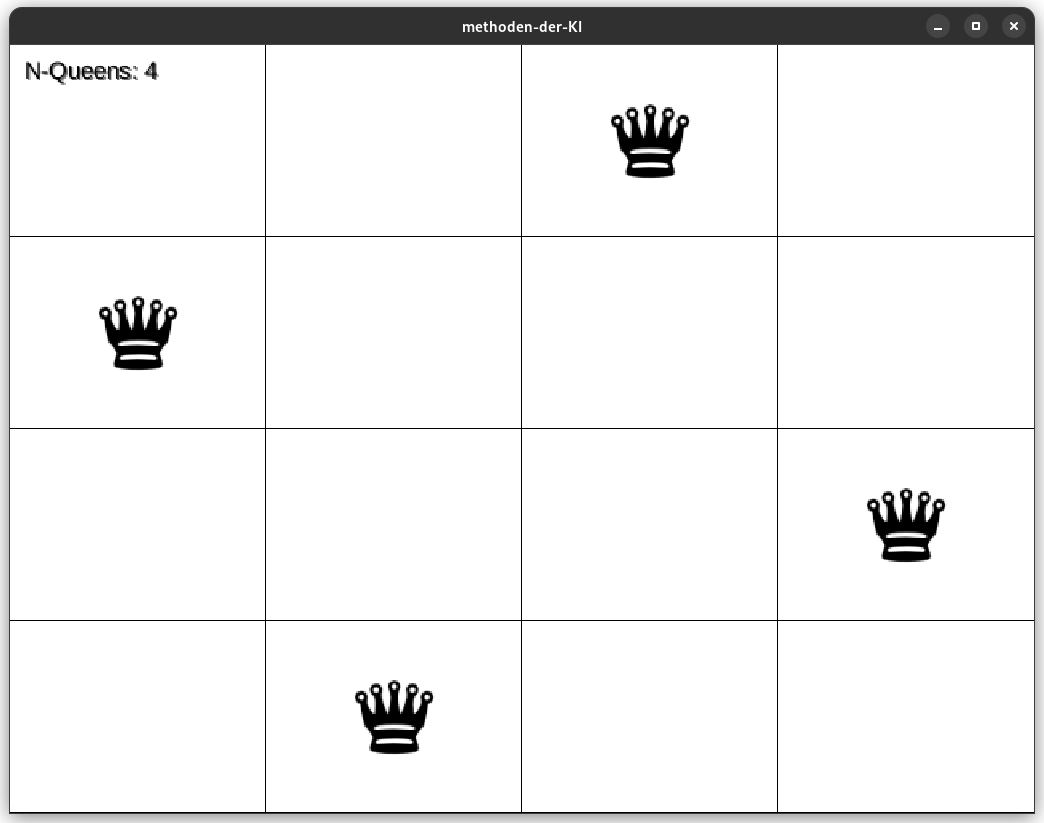
\includegraphics[width=0.8\textwidth]{figures/kap5/n-queens-impl.png}
    \caption{N-Damen Implementierung mit n=4}
    \label{fig:impl-n-damen}
\end{figure}

In diesem Programm wird das n-Damen-Problem f�r n=4 bis 27 unter Verwendung von Constraints gel�st. In diesem Programm w�rde das Dr�cken der Aufw�rts- und Abw�rtspfeiltasten den Wert von N entsprechend erh�hen oder verringern. Das Gitter aktualisiert sich dann selbst, um n x n beizubehalten, und der Choco-Cosntraintssl�ser wird jedes Mal verwendet, wenn sich n �ndert, um eine L�sung zu generieren. Das Programm funktioniert f�r Werte von n von 4 bis 27, aber da die Gr��e des Damenbildes nicht skaliert, ist es schwer zu sehen, wo genau eine Dame nach n=18 platziert wird.

Die Tastensteuerungen wie folgt:
\begin{itemize}
    \item \textbf{Up Arrow Key:} Erh�ht den Wert von N.
    \item \textbf{Down Arrow Key:} Verringert den Wert von N.
    \item \textbf{Escape-Taste:} Geht zur�ck zum Start-Screen.
\end{itemize}

Der relevante Code f�r das Programm befindet sich in den folgenden Packages:
\begin{itemize}
    \item \textbf{de.augsburg.hs.methoden.ki.algorithms.constraints:} Implementierung der Constraints mit Choco-Solver.
    \item \textbf{de.augsburg.hs.methoden.ki.screens.minmax} Klasse f�r den N-Queen-Screen.
    \item \textbf{de.augsburg.hs.methoden.ki.actors.nqueens:} Klassen f�r die Darstellung der Damen.
\end{itemize}

\input{kapitel/5/kap_5.3.tex}

\input{kapitel/5/kap_5.4.tex}